%!TEX program = xelatex
%%%%%%%%%%%%%%%%%%%%%%%这是导言部分的开始%%%%%%%%

%========= 导言部分声明文档的类型=================
\documentclass{article}

%=========导言部分可可以加载宏包=================
\usepackage{amsmath}                % 数学公式排版宏包
\usepackage{amssymb}                % 数学符号命令宏包
\usepackage{amsthm}                 % 数学定理宏包
\usepackage[UTF8]{ctex}             % 中文输入宏包
\usepackage[a4paper]{geometry}      % 页面设置宏包
\usepackage{setspace}               % 行间距宏包
\usepackage{graphicx}               % 图片宏包
\usepackage{listings}               % 代码宏包
\usepackage{color}					% 颜色宏包
\usepackage{xcolor}                 % 颜色处理宏包
\usepackage{float}                  % 浮动对象式样宏包
\usepackage{fontspec}
\usepackage{enumerate}				% 列举编号包

%=========页面设置==============================
\geometry{left=1cm,right=1cm,top=1cm,bottom=2cm}
\onehalfspacing
\setlength\parindent{0em}

%=========代码格式设置============================
\definecolor{dkgreen}{rgb}{0,0.6,0}
\definecolor{gray}{rgb}{0.5,0.5,0.5}
\definecolor{mauve}{rgb}{0.58,0,0.82}
% \setmonofont{Consolas}
\lstset{
	numbers = left, 	
	numberstyle = \color{gray}, 
	keywordstyle = \color{blue},
	commentstyle = \color{dkgreen}, 
	stringstyle = \color{mauve},
	basicstyle = \ttfamily,
	breaklines = true,
	frame = shadowbox, % 阴影效果
	rulesepcolor = \color{ red!20!green!20!blue!20} ,
	escapeinside = ``, % 英文分号中可写入中文
	xleftmargin = 2em,xrightmargin=2em, aboveskip=1em,
	framexleftmargin = 2em
} 

%=========导言部分可以定义标题信息===============
\title{组会报告}
\author{徐益}
\date{\today}
%%%%%%%%%%%%%%%%%%%%%%%这是导言部分的结束%%%%%%%%%

%%%%%%%%%%%%%%%%%%%%%%%这是正文部分的开始%%%%%%%%%
\begin{document}

%=========生成标题================================
\maketitle

%=========开始正文的输入==========================

%===========第一节=================
\section{工作内容} 
1. 解决基于C的5GNR自适应调制编码参数测试平台中的Bug;

2. 更新各CQI的门限SNR;

3. 测试通过交换机的DPDK传输;

4. 配置服务器编译环境。

%===========第二节=================
\section{测试平台Bug的解决}
\subsection{Bug1:向上取整的错误}
\lstset{language=C++}
\begin{lstlisting}
mapped_len = (G + 1) / Q - 1;
改为
mapped_len = (G - 1) / Q + 1;
\end{lstlisting}
\subsection{Bug2:译码矩阵长度选择偏小}
\lstset{language=C++}
\begin{lstlisting}
col_hbg_d = K_b * 1024 / R + 2;
col_hbg_d = col_hbg_d >= (K_b + 4) ? col_hbg_d : (K_b + 4);
col_hbg_d = col_hbg_d <= col_hbg ? col_hbg_d : col_hbg;
改为
col_hbg_d = K_b * 1024 / R + 3;
col_hbg_d = col_hbg_d >= (K_b + 4) ? col_hbg_d : (K_b + 4);
col_hbg_d = col_hbg_d <= col_hbg ? col_hbg_d : col_hbg;
\end{lstlisting}
\subsection{Bug3:快速解调算法造成的性能损失}
\begin{figure}[H]
	\centering
	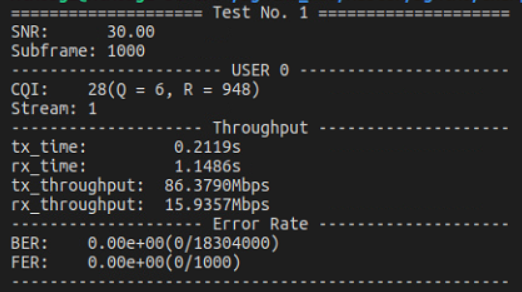
\includegraphics[width = .65\textwidth]{lowdemap.png}
	\caption{理想解调下的时延情况}
\end{figure}
\begin{figure}[H]
	\centering
	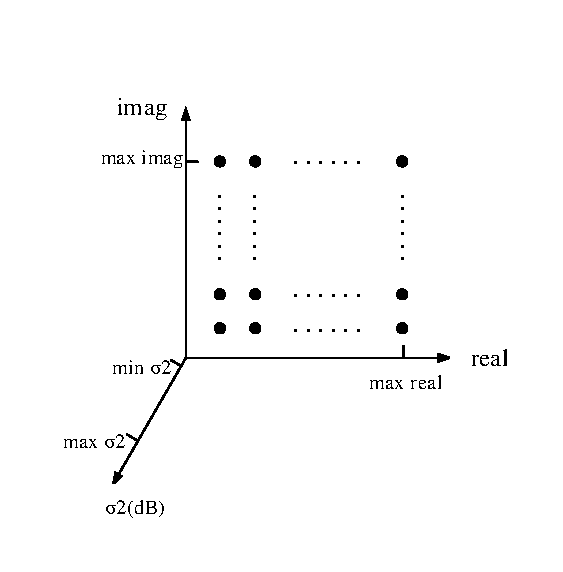
\includegraphics[width = .8\textwidth]{fastmap.pdf}
	\caption{快速解调算法原理}
\end{figure}
\lstset{language=C++}
\begin{lstlisting}
const float symbol_max[3] = {0.7071 * 2, 0.9487 * 2, 1.0801 * 2};
float sigma_max = log10(1);
int SymbOrder = 6;
int SigmaOrder = 4;
改为
const float symbol_max[3] = {0.7071 * 4, 0.9487 * 4, 1.0801 * 4};
float sigma_max = log10(10);
int SymbOrder = 7;
int SigmaOrder = 5;
\end{lstlisting}

%===========第三节=================
\section{更新后的各CQI的门限SNR}
\begin{table}[H]
	\caption{不同CQI的门限SNR值}
	\centering
	\begin{tabular}{|l|l|l|l|l|l|l|}% 通过添加 | 来表示是否需要绘制竖线
		\hline  % 在表格最上方绘制横线
		CQI		& Q		& R		& $SNR_{th}$(dB)(理想)	& $SNR_{th}$(dB)(调整前)	& $SNR_{th}$(dB)(调整后)	\\
		\hline
		0		& 2		& 120	& -5.28	& -3.00	& -5.44 \\
		\hline
		1		& 2		& 157	& -4.29	& -2.45	& -4.33 \\
		\hline
		2		& 2		& 193	& -3.24	& -1.94	& -3.30 \\
		\hline
		3		& 2		& 251	& -1.94	& -1.26	& -2.15 \\
		\hline
		4		& 2		& 308	& -0.86	& -0.61	& -1.03 \\
		\hline
		5		& 2		& 379	&  0.22	& 0.19	& 0.11 \\
		\hline
		6		& 2		& 449	&  1.09	& 0.97	& 0.94 \\
		\hline
		7		& 2		& 586	&  1.98	& 1.79	& 1.88  \\
		\hline
		8		& 2		& 602	&  2.85	& 2.81	& 2.69  \\
		\hline
		9		& 2		& 679	&  3.73	& 3.64	& 3.63  \\
		\hline
		10		& 4		& 340	&  4.38	& 5.39	& 4.59  \\
		\hline
		11		& 4		& 378	&  4.98	& 5.39	& 5.15  \\
		\hline
		12		& 4		& 434	&  5.89	& 5.98	& 6.18  \\
		\hline
		13		& 4		& 490	&  6.75	& 7.17	& 6.87  \\
		\hline
		14		& 4		& 553	&  7.64	& 7.99	& 7.79  \\
		\hline
		15		& 4		& 616	&  8.59	& 8.68	& 8.80 \\
		\hline
		16		& 4		& 658	&  9.20	& 9.44	& 9.38 \\
		\hline
		17		& 6		& 438	& 10.41	& 10.69	& 10.97 \\
		\hline
		18		& 6		& 466	& 10.89	& 10.97	& 11.00 \\
		\hline
		19		& 6		& 517	& 11.77	& 12.44	& 12.18 \\
		\hline
		20		& 6		& 567	& 12.60	& 13.39	& 12.69 \\
		\hline
		21		& 6		& 616	& 13.55	& 13.61	& 13.86 \\
		\hline
		22		& 6		& 666	& 14.34	& 14.66	& 14.47 \\
		\hline
		23		& 6		& 719	& 15.35	& 15.70	& 15.54 \\
		\hline
		24		& 6		& 772	& 16.22	& 16.38	& 16.36 \\
		\hline
		25		& 6		& 822	& 17.08	& 17.32	& 17.32 \\
		\hline
		26		& 6		& 873	& 18.06	& 18.64	& 18.36 \\
		\hline
		27		& 6		& 910	& 18.89	& 19.22	& 19.19 \\
		\hline
		28		& 6		& 948	& 20.11	& 20.57	& 20.56 \\
		\hline  % 在表格最下方绘制横线
	\end{tabular}
\end{table}

%===========第四节=================
\section{测试通过交换机的DPDK传输}
\begin{figure}[H]
	\centering
	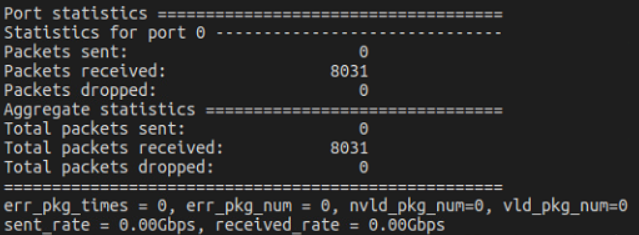
\includegraphics[width = .8\textwidth]{switch_err.png}
	\caption{收到交换机中的无效包}
\end{figure}
\begin{figure}[H]
	\centering
	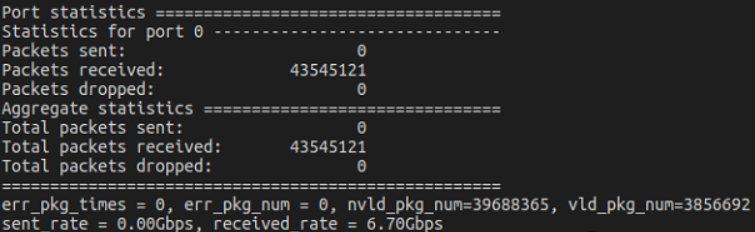
\includegraphics[width = .8\textwidth]{switch.png}
	\caption{增加MAC地址检测后正常接收}
\end{figure}

%===========第五节=================
% \section{有PRACH情况下的资源分配问题}
% \begin{figure}[H]
% 	\centering
% 	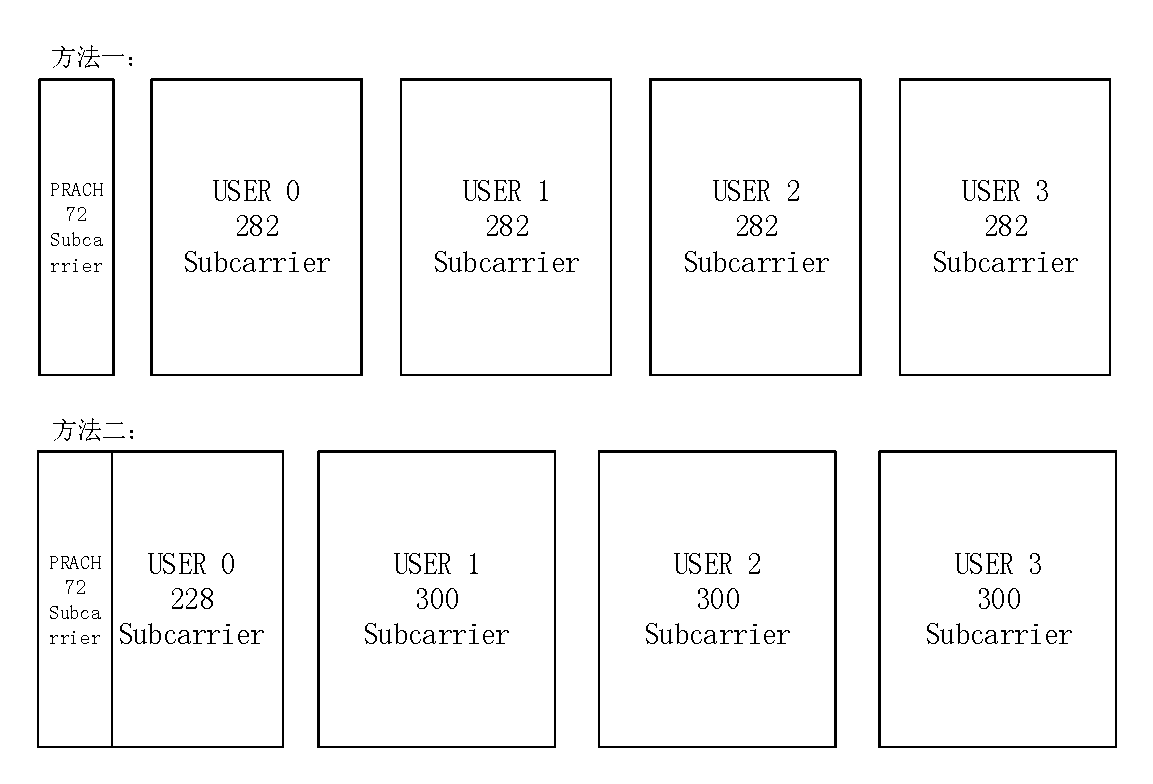
\includegraphics[width = \textwidth]{ques.pdf}
% 	\caption{两种方案}
% \end{figure}

%===========下周计划=================
% \section{下阶段计划}
% 1. 完善单线程系统(修复Bug)

\end{document}
%%%%%%%%%%%%%%%%%%%%%%%这是正文部分的结束%%%%%%%%%%%%